\PID 
Нека је дат дискретан сигнал $x[n] = \cos(\Omega_0 n)$, чији је основни период $N_0 = 10$. Применом 
Фуријеове траснформације дискретног сигнала, скицирати развој датог сигнала у Фуријеов ред 
$X[k] = \FS{x[n]}$ на дужини (а) $N_{\rm F} = N_0$ и (б) $N_{\rm F} = N_0 - 1$. \\

\textsc{\underline{Решење}:} Веза између Фуријеове трансформације сигнала $x[n]$, дужине $N_F$, и Фуријеовог реда 
периодичног продужења истог сигнала, $\hat x[n]$, дата је у облику 
\begin{equation}
    \hat X[k] = \dfrac{1}{N_F} X(\jj k \Omega_{\rm F}), \qquad \Omega_{\rm F} = \dfrac{2\uppi}{N_{\rm F}} \label{\ID.dtfs_dtft}
\end{equation}
На сличан начин као у задатку \ref{z:dso}, представимо дати сигнал као $x[n] = \cos(\Omega_0 n) \rect_{\dfrac{N_{\rm F}-1}2}[n]$.
Онда је Фуријеова трансформација тог сигнала (према резултату истог задатка) једнака
\begin{equation}
    X(\jj\Omega)
    =
    \dfrac{1}{2} \left(
    \dfrac{\sin( (\Omega - \Omega_0)(N + 0,5) ) }{ \sin((\Omega - \Omega_0)/2) }
    +
    \dfrac{\sin( (\Omega + \Omega_0)(N + 0,5) ) }{ \sin((\Omega + \Omega_0)/2) }  \right), \qquad N = \dfrac{N_{\rm F}-1}{2}
\end{equation}
На основу резултата \ref{\ID.dtfs_dtft}, добија се тражени Фуријеов ред 
\begin{equation}
    \hat X[k] = 
    X(\jj k \Omega_{\rm F} )
    =
    \dfrac{1}{2N_{\rm F}}
    \left(
    \dfrac{\sin( (k \Omega_{\rm F} - \Omega_0)(N + 0,5) ) }{ \sin((k \Omega_{\rm F} - \Omega_0)/2) }
    +
    \dfrac{\sin( (k \Omega_{\rm F} + \Omega_0)(N + 0,5) ) }{ \sin((k \Omega_{\rm F} + \Omega_0)/2) }
    \right).
\end{equation}

(а) Када је $N_{\rm F} = N_0$, односно $\Omega_{\rm F} = \Omega_0$, може се даље писати да је 
\begin{eqnarray}
    \dfrac{\sin( (k \Omega_{\rm F} \pm \Omega_0)(N + 0,5) ) }{ \sin((k \Omega_{\rm F} \pm \Omega_0)/2) }
    = 
    \dfrac{\sin \left( (k \Omega_{\rm 0} \pm \Omega_0) \dfrac{\uppi}{\Omega_0} \right) }{ \sin((k \Omega_{\rm 0} \pm \Omega_0)/2) } 
    = \dfrac{ \sin \bigl( (k \pm 1)\uppi \bigr) }{ \sin \left( (k \pm 1)\dfrac{\Omega_0}2 \right)},
\end{eqnarray}
којом приликом знак „$-$“ одговара првом а знак „$+$“ другом сабиркуу коначном изразу.
Са друге стране, у интервалу од интереса $ 0 \leq k < N_{0}$ (основни период дискретног спектра) важи да је 
\begin{eqnarray}
    \dfrac{ \sin \bigl( (k \pm 1)\uppi \bigr) }{ \sin \left( (k \pm 1)\dfrac{\Omega_0}2 \right)} = 
    \begin{cases}
        \dfrac{2\uppi}{\Omega_0} = N_0 &, k \pm 1 = 0, \\
        0 &, k \pm 1 \neq 0.
    \end{cases}
\end{eqnarray}
На основу добијеног резултата, наведени сабирак представља дискретан јединични импулс, 
$N_0 \updelta[k \pm 1]$, па је у овом случају тражени спектар
\begin{equation}
    \hat X[k] = \dfrac{1}{2}\updelta[k + 1] + \dfrac{1}{2}\updelta[k - 1],
\end{equation}
што је исти резултат који се може добити на сличан начин као и у задатку \ref{z:DTFS_sin} на основу непосредне примене резултата
$\sin({\Omega n}) = \dfrac{1}{2} \ee^{\jj\Omega n} + \dfrac{1}{2} \ee^{-\jj\Omega n}$.

(б) Сличан поступак се може спровсети и у случају када $N_{\rm F} \neq N_0$. У том случају, ипак, решење неће имати нуле на местима када је 
$k \pm 1 = 0$. Поједностављење добијеног израза препуштамо читаоцу. 

Резултати (а) и (б) приказани су на сликама \ref{\ID.fig.a} и \ref{\ID.fig.b}. 
Појава која се може видети јесте \textit{цурење спектра}, које је значајна последица јер се увек помоћу дигиталног рачунара 
може вршити само израчунавање Фуријеовог реда коначно дугачке секвенце.


\begin{figure}[ht!]
    \begin{subfigure}{0.49\textwidth}
        \centering
        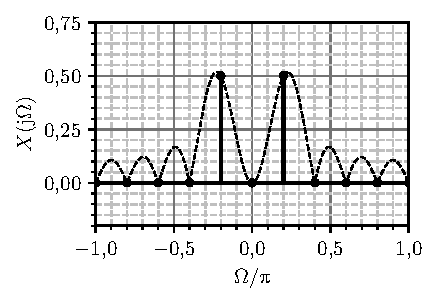
\includegraphics[scale=1]{fig/sample_X_noleak.pdf}
        \caption{$N_{\rm F} = N_{0}$}
        \label{\ID.fig.a}
    \end{subfigure}
    %
    \begin{subfigure}{0.49\textwidth}
        \centering
        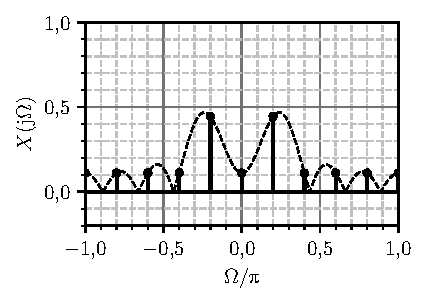
\includegraphics[scale=1]{fig/sample_X_leak.pdf}
        \caption{$N_{\rm F} = N_{0}-1$}
        \label{\ID.fig.b}
    \end{subfigure}
    \caption{Графички приказ одабирања спектра.}
\end{figure}